\section{Low-cost Cuts via Ball-Growing}

It will be useful for us to develop some more machinery to discuss the volume of a ball as well as the cost of the partitions added to $F$. Let us define the following.
\vspace{-1em}
\begin{enumerate}[(1)]
\item Define the total volume of the given graph to be $V^*$ given by
\begin{equation*}
V^* = \sum_{e \in E} c_e x_e
\end{equation*}

Since $x$ is the LP optimal solution, $V^*$ lower bounds the cost of the optimal multicut $\opt$.

\item Previously, we defined the volume of a ball $\text{Vol} \; \mathcal{B}_x(u', r)$. Let us now denote another quantity $V_x(s_i, r)$ as the volume of $\mathcal{B}_x(s_i, r)$ with an added $\frac{V^*}{k}$ term.
\begin{equation*}
V_x(s_i, r) = \frac{V^*}{k} + \text{Vol} \; \mathcal{B}_x(s_i, r)
\end{equation*}

The $\frac{V^*}{k}$ term seems a bit mysterious, but adding this term ensures two properties. First, $V_x(s_i, 0) > 0$ for all $i = 1, \ldots, k$ since $\frac{V^*}{k} > 0$. Second, we have
\begin{equation*}
\sum_{i=1}^k V_x(s_i, 0)
= \sum_{i=1} \frac{V^*}{k}
= V^*
\end{equation*}

These two properties will be quite handy later.

\item Define $c_x(s_i, r)$ to be the cost of the cut induced by removing $\mathcal{B}_x(s_i, r)$ from the graph. That is
\begin{equation*}
c_x(s_i, r) = \sum_{e \in \partial(\mathcal{B}_x(s_i, r))} c_e
\end{equation*}
\end{enumerate}

% --------------------------------------------------------------------
% BALL-GROWING
% --------------------------------------------------------------------

\subsection{Ball-Growing}

Consider a the ball $\mathcal{B}(s_i, r)$ removed during an iteration of algorithm~\ref{alg:rounding}. It is uncertain how we can handle the cost of cut $\partial(\mathcal{B}(s_i, r))$ directly, but suppose we could \emph{charge} the cost of the cut to the volume of the ball. That is to say we could discover $\alpha$ such that
\begin{equation}\label{eqn:target-ineq}
c_x(s_i, r) \leq \alpha \cdot V_x(s_i, r)
\end{equation}

This would be very useful as we would then have a potential way to relate the cost of the cut to $V^*$ a lowerbound on $\opt$. The reason why we can expect such an $\alpha$ to exist, and also why pipe networks provide such a nice analogy for this problem, is because the change in volume of a pipe captured by an infinitesimal change in the radius of the ball is proportional to the pipe's cross-sectional area. That is to say:
\begin{equation*}
V_x'(s_i, r) = \frac{d}{dr} V_x(s_i, r) = c_x(s_i, r)
\end{equation*}

Imagine a ball around $s_i$ like so. If we grow $r$ by an infinitesimally small amount then we add the sum of cross-sectional area of all pipes crossing the boundary $\mathcal{B}(s_i, r)$ to the volume of $\mathcal{B}(s_i, r)$. The sum of cross-sectional areas of pipes crossing the boundary of $s_i$'s ball is exactly the quantity measured by $c_x(s_i, r)$!

\begin{figure}[h!]
    \centering
    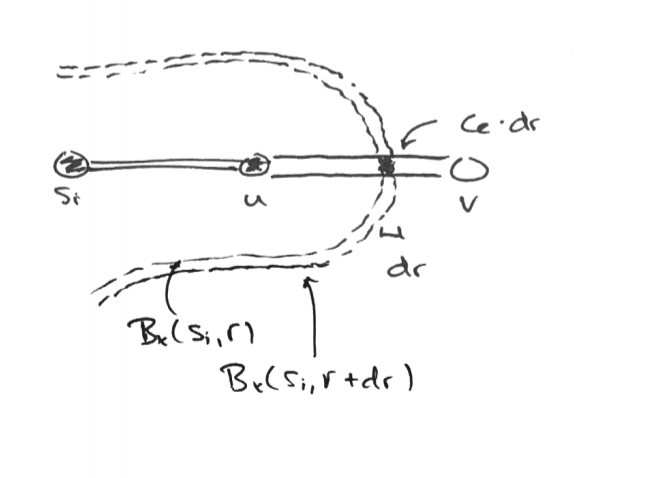
\includegraphics[scale=0.6]{images/image-3.png}
\end{figure}
\vspace{-1em}
Inequality~\ref{eqn:target-ineq} would then reduce to the following
\begin{equation*}
c_x(s_i, r) \leq \alpha \cdot V_x(s_i, r)
\qquad\Longrightarrow\qquad
\frac{c_x(s_i, r)}{V_x(s_i, r)} \leq \alpha
\qquad\Longrightarrow\qquad
\frac{V_x'(s_i, r)}{V_x(s_i, r)} \leq \alpha
\end{equation*}

But $\frac{V_x'(s_i, r)}{V_x(s_i, r)}$ is the derivative of $\ln (V_x'(s_i, r))$. If we let $F'(r) = \frac{V_x'(s_i, r)}{V_x(s_i, r)}$, we can reduced our task of determining $\alpha$ to bounding the value of derivative of $F(r)$. For that we use the Mean Value Theorem. If $F(r)$ is continuous on $[a, b]$ and differentiable on $(a, b)$, then there exists $c \in (a, b)$ such that
\begin{equation*}
F'(c) = \frac{F(b) - F(a)}{b - a}
\end{equation*}

However, $F$ is a monotonic non-increasing function. Thus we have for any $r \in [0, \frac{1}{2})$
\begin{equation*}
F'(r)
\leq \frac{F(\frac{1}{2}) - F(0)}{\frac{1}{2} - 0}
\end{equation*}

Let's first bound $F(\frac{1}{2})$. The volume of any ball of radius $r$ will be at most the total volume of the graph, hence we have the following.
\begin{equation*}
F\bigg( \frac{1}{2} \bigg)
= \ln \bigg( V_x \bigg( s_i, \frac{1}{2} \bigg) \bigg)
\leq \ln\bigg(V^* + \frac{V^*}{k}\bigg)
\end{equation*}

Then we bound $F(0)$. This is where it's critical that $V_x(s_i, 0) > 0$, otherwise the logarithm is undefined!
\begin{equation*}
F(0) = \ln(V_x(s_i, 0)) = \ln\bigg( \frac{V^*}{k} \bigg)
\end{equation*}

We can now bound $F'(r)$. We have
\begin{equation*}
\frac{c_x(s_i, r)}{V_x(s_i, r)}
= F'(r)
\leq \frac{F(\frac{1}{2}) - F(0)}{\frac{1}{2} - 0}
\leq 2 \bigg( \ln\bigg(V^* + \frac{V^*}{k}\bigg) - \ln\bigg( \frac{V^*}{k} \bigg) \bigg)
= 2 \ln(k + 1)
\end{equation*}

What we have shown is that, for an auspicious choice of $r$, we can bound the cost our cut with the volume of the cut. The technique of finding such a cut where we can charge the cost of its boundary to the volume is known as \emph{ball-growing}. To summarize, we have demonstrated
\begin{theorem}\label{thm:region-growing}
Given a feasible solution $x$ to LP~\ref{eq:primal-lp}, for any $s_i$ there exists an $r \in [0, \frac{1}{2})$ that can be found in polynomial time such that
\begin{equation*}
\textup{cost}(\partial(\mathcal{B}_x(s_i, r))) \leq 2 \ln(k+1) \cdot V_x(s_i, r)
\end{equation*}
\end{theorem}

Except we haven't really demonstrated this. The application of the Mean Value Theorem requires $F$ to be differentiable. However, $F(r)$ may not even be continuous at certain points! We will fix this issue with a more careful application of the Mean Value Theorem and also demonstrate how $r$ can be found in polynomial time later on in the notes. For now, let's suppose we have theorem~\ref{thm:region-growing} and complete our analysis of the approximation ratio.

% --------------------------------------------------------------------
% THE APPROXIMATION RATIO
% --------------------------------------------------------------------

\subsection{The Approximation Ratio}

Our heuristic argument in the preceding section demonstrates the existence of an $r$ such that the cost of a ball is at most $2 \ln(k+1)$ times its volume. Using this, we'll show that algorithm~\ref{alg:rounding} returns a $4 \ln(k+1)$-approximation.

\begin{theorem}\label{thm:approx-ratio}
Algorithm~\ref{alg:rounding} returns a $4 \ln(k+1)$-approximation for multicut
\end{theorem}
\begin{proof}
At each iteration of algorithm~\ref{alg:rounding}, we add $F_i = \partial(\mathcal{B}_x(s_i, r))$ to $F$. In iterations $i$ where no ball is removed, we'll let $F_i = \varnothing$ and $\text{Vol} \; \mathcal{B}_x(s_i, r) = 0$. Choosing $r$ according to theorem~\ref{thm:region-growing} gives the cost of $F_i$.
\begin{equation*}
\textup{cost}(F_i)
\leq 2 \ln(k+1) \cdot V_x(s_i, r)
= 2 \ln(k+1) \cdot \bigg( \text{Vol} \; \mathcal{B}_x(s_i, r) + \frac{V^*}{k} \bigg)
\end{equation*}

Since $\mathcal{B}_x(s_i, r)$ is removed from $G$ at every iteration along with all adjacent edges, $F_i \cap F_j = \varnothing$ for $i \neq j$. Additionally, the volume measured by $\text{Vol} \; \mathcal{B}_x(s_i, r)$ will not overlap with that measured by $\text{Vol} \; \mathcal{B}_x(s_j, r)$ for $i \neq j$. The total cost of $F$ returned by the algorithm is the following.
\begin{align*}
\textup{cost}(F)
&= \sum_{i=1}^k \textup{cost}(F_i) \\
&\leq 2 \ln(k+1) \cdot \sum_{i=1}^k \bigg( \text{Vol} \; \mathcal{B}_x(s_i, r) + \frac{V^*}{k} \bigg) \\
&= 2 \ln(k+1) \cdot \big( V^* + V^* \big) \\
&= 4 \ln(k+1) \cdot V^*
\end{align*}

and because $V^*$ is the cost of the optimal LP solution $x$, which lower bounds the optimal cost $\opt$ of any multicut, we have $\textup{cost}(F) \leq 4 \ln(k+1) \cdot \opt$ as required.
\end{proof}

% --------------------------------------------------------------------
% CONTINUITY ISSUES
% --------------------------------------------------------------------

\subsection{Fixing Continuity Issues}

Let's revisit the continuity of $F(r) = \ln(V_x(s_i, r))$ and ask where $F(r)$ could be discontinuous. Around where $r = d_x(s_i, u)$ for some vertex $u \neq s_i$, there could be a discontinuous jump in $V_x(s_i, r)$ because $u$ could be connected to more than one pipe not currently in $\mathcal{B}_x(s_i, r)$.
\begin{figure}[h!]
    \centering
    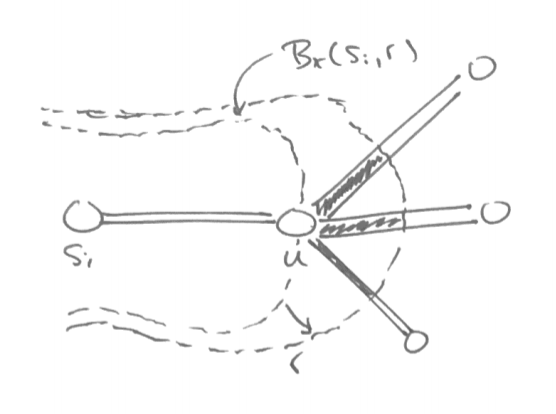
\includegraphics[scale=0.6]{images/image-2.png}
\end{figure}
\vspace{-1em}

However, on intervals of $r \in [0, \frac{1}{2})$ where increasing $r$ does not introduce a new vertex into $\mathcal{B}_x(s_i, r)$, the value of $V_x(s_i, r)$ grows smoothly with respect to $r$. This suggests that we should partition the interval $[0, \frac{1}{2})$ into intervals where \emph{no new vertex} is introduced into $\mathcal{B}_x(s_i, r)$. We now prove theorem~\ref{thm:region-growing}.

\begin{proof}[Proof of theorem~\ref{thm:region-growing}]
We will show that there exists $r \in [0, \frac{1}{2})$ such that
\begin{equation*}
\frac{c_x(s_i, r)}{V_x(s_i, r)} \leq 2 \ln(k+1)
\end{equation*}

Let us order the vertices $v \neq s_i$ as $v_1, \ldots, v_{\ell}$ where
\begin{equation*}
d_x(s_i, v_{j_1}) \leq d_x(s_i, v_{j_2})
\end{equation*}

when $j_1 \leq j_2$, define $r_j = d_x(s_i, v_j)$, and denote $r_j^-$ as value that's infinitesimally smaller than $r_j$. We will demonstrate the existence of $r$ by choosing it uniformly at random on the interval $[0, \frac{1}{2})$. If we can bound the \emph{expectation} of $\frac{c_x(s_i, r)}{V_x(s_i, r)}$ by what we want, then there must exist an actual choice of $r$ where the bound holds deterministically. Our choice of partitioning $[0, \frac{1}{2})$ using $r_j$'s is critical as $F(r)$ is continuous over interval $[r_j, r_{j+1}^{-}]$ and differentiable over $(r_j, r_{j+1}^-)$. For notational simplicity, let $r_{\ell + 1} = \frac{1}{2}$. Let us compute the expectation of $\frac{c_x(s_i, r)}{V_x(s_i, r)}$ when $r$ is distributed uniformly at random on $[0, \frac{1}{2})$.
\begin{align*}
\mathbb{E} \bigg[ \frac{c_x(s_i, r)}{V_x(s_i, r)} \bigg]
&= \frac{1}{\frac{1}{2} - 0} \cdot \int_0^{\frac{1}{2}} \frac{c_x(s_i, r)}{V_x(s_i, r)} \; dr \\
&= \frac{1}{\frac{1}{2} - 0} \cdot \sum_{j = 1}^{\ell} \int_{r_j}^{r_{j+1}^-} \frac{c_x(s_i, r)}{V_x(s_i, r)} \; dr \\
&= 2 \cdot \sum_{j=1}^\ell \Big( \ln(V_x(s_i, r^-_{j+1})) - \ln(V_x(s_i, r_{j})) \Big) \\
&\leq 2 \cdot \sum_{j=1}^\ell \Big( \ln(V_x(s_i, r_{j+1})) - \ln(V_x(s_i, r_{j})) \Big)
\end{align*}

The last line follows as $F(r)$ is monotonically non-decreasing. This forms a telescoping sum which reduces to
\begin{equation*}
2 \cdot \sum_{j=1}^\ell \Big( \ln(V_x(s_i, r_{j+1})) - \ln(V_x(s_i, r_{j})) \Big)
= 2 \cdot \Big( \ln(V_x(s_i, \tfrac{1}{2})) - \ln(V_x(s_i, 0)) \Big)
\leq 2 \ln(k+1)
\end{equation*}

Consequently, the expectation is bounded by $2 \ln(k+1)$ hence there must be an $r$ achieving $\frac{c_x(s_i, r)}{V_x(s_i, r)} \leq 2 \ln(k+1)$. To find $r$ in polynomial time, observe that on the interval $[r_j, r_{j+1}]$ the cost of the boundary $c_x(s_i, r)$ remains constant while $V_x(s_i, r_{j+1})$ grows monotonically. This means the ratio $\frac{c_x(s_i, r)}{V_x(s_i, r)}$ is minimized at $r_{j+1}$. Finding the minimizer requires only checking each $r_1, \ldots, r_{\ell}$, and as $\ell \leq n$, a linear number of computations suffice.
\end{proof}
